\documentclass[14pt]{beamer}
\usepackage[T2A]{fontenc}
\usepackage[utf8]{inputenc}
\usepackage[english]{babel}
\usepackage{amssymb,amsfonts,amsmath,mathtext}
\usepackage{cite,enumerate,float,indentfirst}
\usepackage{verbatim,longtable}

\graphicspath{{../Dissertation/images/}}

\beamertemplatenavigationsymbolsempty

%%% Основные сведения %%%
\newcommand{\thesisAuthorLastName}{{Lazarenko}}
\newcommand{\thesisAuthorOtherNames}{{Denys}}
\newcommand{\thesisAuthorInitials}{{D.\,L.}}
\newcommand{\thesisAuthor}             % Диссертация, ФИО автора
{%
    \texorpdfstring{% \texorpdfstring takes two arguments and uses the first for (La)TeX and the second for pdf
        \thesisAuthorLastName~\thesisAuthorOtherNames% так будет отображаться на титульном листе или в тексте, где будет использоваться переменная
    }{%
        \thesisAuthorLastName, \thesisAuthorOtherNames% эта запись для свойств pdf-файла. В таком виде, если pdf будет обработан программами для сбора библиографических сведений, будет правильно представлена фамилия.
    }
}
\newcommand{\thesisAuthorShort}        % Диссертация, ФИО автора инициалами
{\thesisAuthorInitials~\thesisAuthorLastName}
%\newcommand{\thesisUdk}                % Диссертация, УДК
%{\todo{xxx.xxx}}
\newcommand{\thesisTitle}              % Диссертация, название
{{Text Classification with Deep Learning}}
\newcommand{\thesisSpecialtyNumber}    % Диссертация, специальность, номер
{{124}}
\newcommand{\thesisSpecialtyTitle}     % Диссертация, специальность, название
{{System analysis and control}}
\newcommand{\thesisDegree}             % Диссертация, ученая степень
{{bachelor of System analysis}}
\newcommand{\thesisDegreeShort}        % Диссертация, ученая степень, краткая запись
{{bachelor of System analysis}}
\newcommand{\thesisCity}               % Диссертация, город написания диссертации
{{Kyiv}}
\newcommand{\thesisYear}               % Диссертация, год написания диссертации
{{2018}}
\newcommand{\thesisOrganization}       % Диссертация, организация
{{MINISTRY OF EDUCATION AND SCIENCE OF UKRAINE

NATIONAL TECHNICAL UNIVERSITY OF UKRAINE
«IGOR SIKORSKY KYIV POLYTECHNIC INSTITUTE»
}}
\newcommand{\thesisOrganizationShort}  % Диссертация, краткое название организации для доклада
{{NTUU "KPI"}}

\newcommand{\thesisInOrganization}     % Диссертация, организация в предложном падеже: Работа выполнена в ...
{{Національному технічному університеті України ``Київському політехнічному інституті імені Ігоря Сікорського''}}

\newcommand{\supervisorFio}            % Научный руководитель, ФИО
{{Anton Maltsev}}
\newcommand{\supervisorRegalia}        % Научный руководитель, регалии
{{Ph.D. in Physico-mathematical Science,~docent}}
\newcommand{\supervisorFioShort}       % Научный руководитель, ФИО
{{A.~Maltsev}}
\newcommand{\supervisorRegaliaShort}   % Научный руководитель, регалии
{{Ph.D. in Physico-mathematical Science,~docent}}
      % Основные сведения

\usetheme{Pittsburgh}
\usecolortheme{whale}

\setbeamercolor{footline}{fg=blue}
\setbeamertemplate{footline}{
	\leavevmode%
	\hbox{%
		\begin{beamercolorbox}[wd=.333333\paperwidth,ht=2.25ex,dp=1ex,center]{}%
			    \thesisAuthorShort, \thesisOrganizationShort
		\end{beamercolorbox}%
		\begin{beamercolorbox}[wd=.333333\paperwidth,ht=2.25ex,dp=1ex,center]{}%
			     \thesisCity, \thesisYear
		\end{beamercolorbox}%
		\begin{beamercolorbox}[wd=.333333\paperwidth,ht=2.25ex,dp=1ex,right]{}%
			p. \insertframenumber{} из \inserttotalframenumber \hspace*{2ex}
		\end{beamercolorbox}}%
		\vskip0pt%
	}
	
	\newcommand{\itemi}{\item[\checkmark]}
	
	\title{\small{\thesisTitle}}
	\author{
		\thesisOrganizationLong\\
		\emph{Speaker:}~\thesisAuthorShort\\%
		\emph{Supervisor:}~\supervisorRegaliaShort~\supervisorFioShort\\%
		%\emph{Supervisor:}~\thesisOrganization\\%
%		\vspace{20pt}%
%		\vspace{20pt}%
	}
	\date{\small{\thesisCity, \thesisYear}}

	
	\begin{document}
		
		\maketitle

				
		\begin{frame}
			\frametitle{Introduction}
			{\textbf{Aim}} of this thesis is building an effective model which have high accuracy and an appropriate speed for classification of advertisements at the e-commerce platform Jiji.ng. \\ 
			\textbf{Object of study} is advertisements at e-commerce platform 
			\\
			\textbf{Subject of study} is classification model for advertisements: 	
		\end{frame}
		
		\begin{frame}
			\frametitle{Relevance of the problem}
				\begin{itemize}
					\item e-commerce sales are quickly increasing
					\item large online e-commerce websites serve millions of users’ requests per day
					\item processes of registrations and purchases as much convenient and fast as possible
					\item users have to make a choice from more than hundred categories
					\item  automatic category prediction is very important in terms of saving moderators' time and as a result, decreasing the number of necessary moderators to process them
				\end{itemize}	
		\end{frame}
		
		\begin{frame}
			\frametitle{Structure of the data files}
				\begin{table}[]
					\centering
					\begin{tabular}{|p{1cm} | p{3cm} | p{5cm} |}
						\hline
						\textbf{lvl2} & \textbf{titles}                  & \textbf{descriptions}                                                                   \\ \hline
					    29   & Clean Toyota Camry 2008 Silver   & Fairly used Toyota 08 Camry with no problems V4 engine fabric seats and interior            \\ \hline
						25   & Look Unique                      & Nice, quality, adorable,unique dress available now, whatsapp me                             \\ \hline
					\end{tabular}
				\end{table}
		\end{frame}
		
		\begin{frame}
			\frametitle{Existing approaches}
			Let`s assume we have the following sentences: \\
			
			\textbf{["The sun is yellow", "The sky is blue"]}\\
			
			Encode words with the Bag-of-words method
			\begin{table} [htbp]
				\centering
				%  \begin{center}
				\begin{tabular}{| p{1cm} || p{1cm} | p{1cm} | p{1cm} | p{2cm} | p{1cm} | p{1cm}l |}
					\hline
					\hline
					Text & \centering the  & \centering sun  & \centering is  &\centering yellow &\centering sky  & \centering  blue & \\
					\hline
					$T_{1}$ &\centering  1   &\centering  1  &\centering  1   &\centering  1 &\centering  0 &\centering 0 &   \\
					$T_{2}$ &\centering  1   &\centering  0  &\centering  1   &\centering  0 &\centering  1 &\centering 1 &   \\
					\hline
					\hline
				\end{tabular}
				%  \end{center}
			\end{table}
			\begin{enumerate}
				\item Naive Bayes 
				%\item k-Nearest Neighbors
				\item Logistic Regression 
				\item Support Vector Machines (SVMs)
				\item Decision Trees and Random Forests
			\end{enumerate}  
		\end{frame}
		
		
		\begin{frame}  
			\frametitle{Embeddings}
			\begin{tabular}{cl}  
				\begin{tabular}{l}
					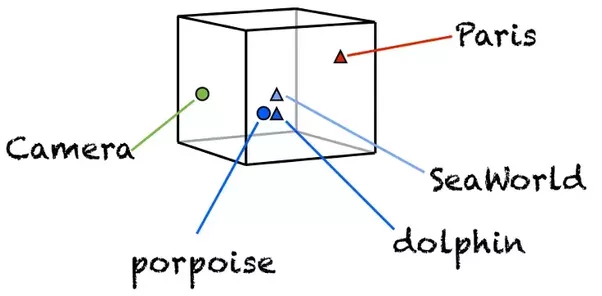
\includegraphics[height=3.5cm, width=5cm]{embed_vectors}
				\end{tabular}
				& \begin{tabular}{l}
					\parbox{0.5\linewidth}{%  change the parbox width as appropiate
						An \textbf{embedding} is a mapping from discrete objects, such as words, to vectors of real numbers. For example, a 300-dimensional embedding for English words could include: \\
						\textbf{blue}: $(0.059, 0.7597, ...)$
					}
				\end{tabular}  \\
			\end{tabular}
		\end{frame}
		
		
		\begin{frame}
			\frametitle{Bi-LSTM Neural Network}
			\begin{table}[h]
				\centering
				\begin{tabular}{| p{4cm} | p{3cm} | p{3cm} |}
					%	\begin{tabulary}{1.0\textwidth}{|L|L|L|L|L|L}
					\hline
					\textbf{Metric}  & \textbf{Train} & \textbf{Test}                                                    
					\\ \hline
					categorical accuracy   &  0.7975 & 0.8203
					\\ \hline
					category crossentropy  &  0.8532 & 0.7478
					\\ \hline
					top k accuracy   &  0.9189 & 0.9219.
					\\ \hline		
				\end{tabular}
			\end{table}	
		\end{frame}
		
		
		\begin{frame}
			\frametitle{Convolution Neural Network }
			\begin{figure}[ht] 
				\center
				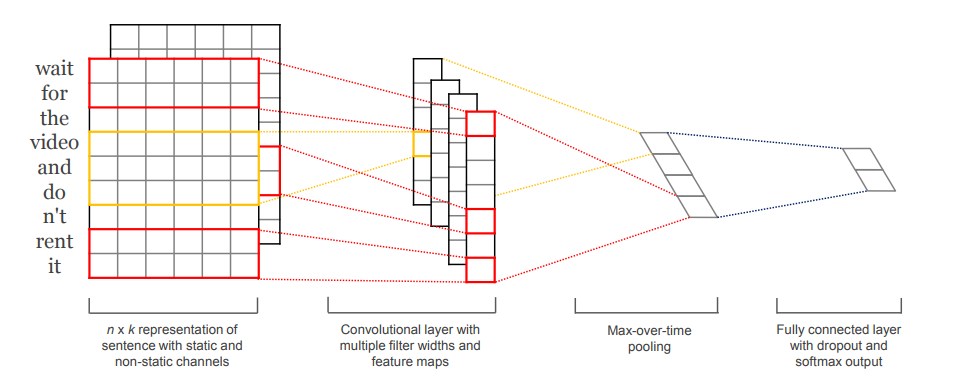
\includegraphics [scale=0.3] {CNN}
			\end{figure}
			\begin{itemize}
				\item 300 filters
				\item size of filter: 3, 4, 5
				\item l2-regularization equals to 0.01 
				\item dropout equals to the rate 0.5
			\end{itemize}	
		\end{frame}
		
		\begin{frame}
			\frametitle{Overfitting}
			\hfil\hfil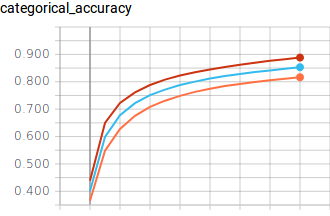
\includegraphics[width=5cm]{part4//3CNN_train_category_accuracy}
			\hfil\hfil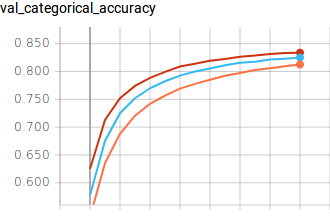
\includegraphics[width=5cm]{part4//3CNN_val_category_accuracy}\newline
			\vfil
			\hfil\hfil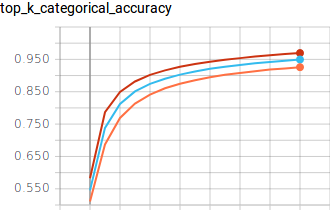
\includegraphics[width=5cm]{part4/3CNN_train_top_k_accuracy}
			\hfil\hfil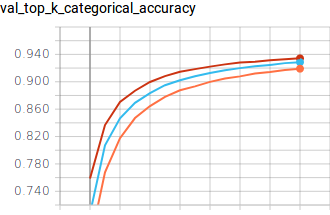
\includegraphics[width=5cm]{part4/3CNN_val_top_k_accuracy}\newline
		\end{frame}
		
		
	\begin{frame}
		\frametitle{Regularizations}
		Modifications:
		\begin{enumerate}
			\item Dropout rate decreased in two times.
			\item l2-regularization equals to 0.01 both for convolution layers and dense layer. 
			Dropout = 0.5 both for dense and convolution layers. 
		    training algorithm - Adam with learning rate 1e-4. 
			\item l2-regularization equals to = rate 1e-3. 
			Dropout = 0.25 both for dense and convolution layers. 
			\item l2-regularization =  0.001 for convolution layers and 0.01 for dense layers. 
			Dropout rate = 0.25 for convolution layers and 0.5 for dense layers.
		\end{enumerate}
	\end{frame}
			
		
		\begin{frame}
			\frametitle{Regularizations}
			\begin{figure}[ht]
				\begin{minipage}[ht]{1\linewidth}
					\center{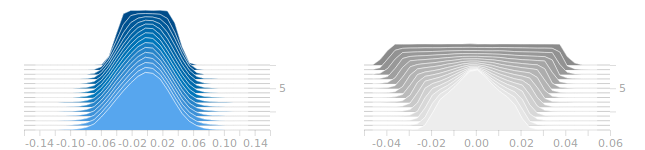
\includegraphics[width=1\linewidth]{part4/4CNN-dense-1.png} \\ а, b}
				\end{minipage}
				\hfill
				\begin{minipage}[ht]{1\linewidth}
					\center{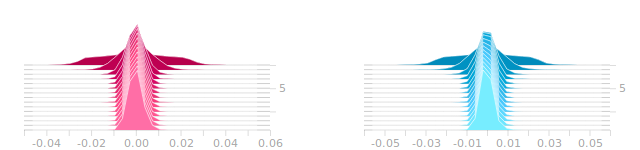
\includegraphics[width=1\linewidth]{part4/4CNN-dense-2.png} \\ c, d}
				\end{minipage}
			\end{figure}
		\end{frame}
		
		\begin{frame}
		\frametitle{Results}
			\hfil\hfil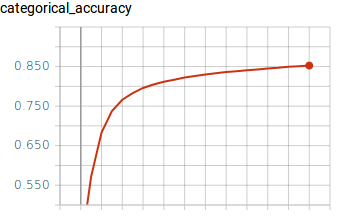
\includegraphics[width=5cm]{part4/final_CNN_train_category_accuracy}
			\hfil\hfil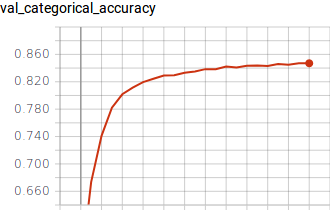
\includegraphics[width=5cm]{part4/final_CNN_val_category_accuracy}\newline
			\vfil
			\hfil\hfil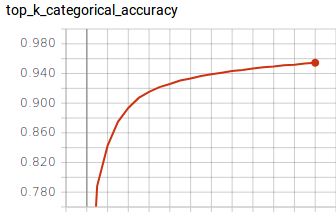
\includegraphics[width=5cm]{part4/final_CNN_train_top_k_accuracy}
			\hfil\hfil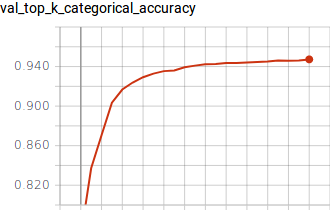
\includegraphics[width=5cm]{part4/final_CNN_val_top_k_accuracy}\newline
		\end{frame}
		
		
		\begin{frame}
			\frametitle{Results}
			\begin{table}[h]
				\centering
				\begin{tabular}{| p{4cm} | p{3cm} | p{3cm} |}
					%	\begin{tabulary}{1.0\textwidth}{|L|L|L|L|L|L}
					\hline
					\textbf{Metric}  & \textbf{Train} & \textbf{Test}                                                    
					\\ \hline
					categorical accuracy   &  0.8250 & 0.8307
					\\ \hline
					category crossentropy  &   0.5800 & 0.6612
					\\ \hline
					top k accuracy   &  0.9545 & 0.9473
					\\ \hline		
				\end{tabular}
			\end{table}
		\end{frame}
		
		\begin{frame}
			\frametitle{Results}
			\begin{longtable}[c]{|l|c|c|l|l|}
				\hline  category & precision & recall &  f1-score & support\\ \hline
				\endhead
				\hline
				\endlastfoot

				11       & 0.78      & 0.58   & 0.66     & 623     \\
				14       & 0.93      & 0.99   & 0.96     & 8070    \\
				15       & 0.82      & 0.68   & 0.74     & 362     \\
				16       & 0.93      & 0.95   & 0.94     & 1656    \\
				20       & 0.82      & 0.91   & 0.86     & 1151    \\
				25       & 0.75      & 0.9    & 0.82     & 1910    \\
				29       & 0.97      & 0.99   & 0.98     & 12346   \\
				\hline
			\end{longtable}
		\end{frame}
		
		\begin{frame}
			\frametitle{Future work}
			\begin{itemize}
				\item train networks with other training algorithms. For example, it is possible
				to try SGD or RMSprop with appropriate parameters;
				\item make an assemble of neural networks to best use each one‘s strong qualities;
				\item try to use different words sequences length for titles and descriptions;
				\item as the results on categories were not really impressive it is possible to add
				them into one large.
			\end{itemize}
		\end{frame}
		

		\begin{frame}
			\begin{center}
					Thank you for your attention!
			\end{center}
		\end{frame}
		
	\end{document} 